\documentclass{scrartcl}
\setkomafont{disposition}{\normalfont\bfseries}
\usepackage[utf8]{inputenc}
\usepackage{graphicx}
\usepackage{hyperref}
\hypersetup{
    colorlinks=true,
    urlcolor=blue,
    filecolor=black,
    linkcolor=black
}
\usepackage{minted}
\usemintedstyle{tango}

\title{Cybernetic Ducks}
\subtitle{Statistics 101C Lecture 4 Final Project Report}
\author{Oscar Monroy, Zoe Wang,\\Christine Marie Castle}
\date{2020-12-14}

\begin{document}

\maketitle

\section{Introduction}

\quad YouTube is the largest online video-sharing platform in the world. A plethora of factors ranging from the duration of the video to the length of the video title to the average pixel value in the thumbnail image could be associated increased engagement. Our goal, simply put, was to find the best model and the optimal set of predictors to successfully predict the success, measured in growth of views between two and six hours after publishing, of any given YouTube video.

\section{Methodology}

\subsection{Preprocessing}

\quad We used the base \verb|R| and \verb|caret| packages to clean the data. We began by looking for any missing values, nonsensical values, or duplicated rows but none were found. The data set did contain several constant variables (i.e. variables with only one unique value); these were eliminated as they provided no information. \verb|id| was removed from the training data set because it contains arbitrary labels that only serve to distinguish the observations. \verb|PublishedDate| was removed because dates are not stored as numeric in \verb|R|, which resulted in errors (e.g. when calculating the correlation matrix).

\subsection{Variable Selection}

\quad We removed highly correlated variables to curb multicollinearity and overfitting. To remove these variables, we used the \verb|findCorrelation| function from the \verb|caret| package, which takes in a correlation matrix and a specified pairwise correlation cutoff (Kuhn, n.d.). It outputs the indices of the variables that have correlations above the cutoff. We removed these variables from the data set.

\begin{figure}
    \centering
    \includegraphics[width=0.75\textwidth]{threshold_vs_rmse.png}
    \caption{Correlation thresholds and corresponding out-of-bag RMSE's}
    \label{fig:thresholds}
\end{figure}

To determine the correlation cutoff, we created five separate data sets with variables removed based on correlation cutoffs of 0.5, 0.6, 0.7, 0.8, and 0.9, and fit a random forest model to each of these sets. We used RMSE and percentage of variance in the response explained, which are both based on predictions on the out-of-bag samples. We considered thresholds no less than 0.5 because we did not want to remove so many variables that our model suffered. The plot in Figure \ref{fig:thresholds} compares the RMSE's with different thresholds. Appendix Table \ref{table:thresholds} shows the percentage of variance explained and optimal \verb|mtry| value (i.e. number of predictors sampled at each split) for each model. The threshold of 0.8 resulted in the lowest RMSE and the highest percentage of variance explained. Using the 0.8 cutoff, we removed 74 variables.

Further, we repeatedly trained a random forest model then used \verb|varImpPlot| in the \verb|randomForest| package to determine and remove variables which were not important to the model. All of the \verb|hog_*| variables and nine other thumbnail features were removed in this process. The final training data set had 73 predictors.

\subsection{Statistical Model}

\quad Our final model was a random forest of 500 trees created with 48 randomly selected predictors considered at each split. To find the optimal \verb|mtry|, we used the \verb|tuneRF| function, which by default started at an \verb|mtry| of \(\left\lfloor\textrm{\#predictors}/3\right\rfloor=24\). The initial \verb|mtry| value is halved multiple times then doubled multiple times, continuing in each direction until model improvement becomes insignificant. \verb|mtry| values and the resulting out-of-bag estimated MSE's are shown in Appendix Figure \ref{fig:oob}.

\begin{table}
    \centering
    \begin{tabular}{| c | c | c |}
         \hline
         Model & Lowest initial CV RMSE estimate & Test RMSE (Kaggle)\\
         \hline
         Random Forest** & 1.48982 & 1.49149\\
         \hline
         Linear Regression & 1.65061 & 1.62673\\
         \hline
         Elastic Net (\(\alpha=0.5\)) & 1.64885 & 1.62927\\
         \hline
         Ridge regression & 1.67215 & 1.63813\\
         \hline
         LASSO regression & 1.67114 & 1.63971\\
         \hline
         PCR* & 2.07693 & ---\\
         \hline
         PLS Regression* & 2.15084 & ---\\
         \hline
    \end{tabular}
    \caption{Lowest cross-validated (out-of-bag for random forest) RMSE estimates of each model we attempted initially. *Predictions were not submitted to Kaggle. **This estimate is not a cross-validated estimate but an out-of-bag estimate}
    \label{table:others}
\end{table}

We decided to pursue a random forest model because the initial RMSE estimate was noticeably less than that of the other models we tried, as shown in Table \ref{table:others}. The RMSE estimates were obtained via 10-fold cross-validation (except for the random forest model, where we had an out-of-bag estimate). For the regularization methods, the shrinkage parameter \(\lambda\) used was chosen from a range of 100 values to minimize the cross-validated RMSE estimate. All of the models were trained on the training data set after removing variables above the 0.8 correlation threshold.

\section{Results}

Our best evaluation metric value with this model as shown in the Kaggle public leaderboard was an RMSE of 1.39935.

\section{Conclusions}

\quad As shown in the Kaggle private leaderboard, the RMSE with this model was 1.41372. One of our models that was trained on more predictors and had a higher public RMSE had a lower private RMSE than this model.

The five most important predictors in our final model (as measured by total decrease in node impurities from splitting on the variable, averaged over all trees) were \verb|Num_Views_Base_mid_high|, \verb|views_2_hours|, \verb|cnn_25|, \verb|cnn_89|, and\\ \verb|Num_Subscribers_Base_mid_high|, as shown in Appendix Figure \ref{fig:varimp}. Three of these predictors relate to how popular the channel or video already is. The other two are thumbnail features.

Our model works well because random forest creates an average of trees that is less variable and thus better at prediction. This is because at each split, random forest considers a random subset of predictors rather than all the predictors unlike bagging. As a result, the trees created are more varied and thus less correlated. Additionally, this reduces test error and the out-of-bag error estimate. Random forest is also computationally inexpensive and easily accessible as the function \verb|tuneRF| takes the work out of optimizing the \verb|mtry| value.

We believe our model could potentially be improved by continuing to analyze the predictors and potentially creating new predictors by combining or transforming predictors.

\pagebreak

\section*{References}

\urlstyle{same}

\quad Kuhn, M. (n.d.). FindCorrelation. Retrieved December 12, 2020, from \url{https://www.rdocumentation.org/packages/caret/versions/6.0-86/topics/findCorrelation}

Liaw, A (n.d.). Importance. Retrieved December 12, 2020, from \url{https://www.rdocumentation.org/packages/randomForest/versions/4.6-14/topics/importance}

\section*{Statement of Contributions}

All members contributed to writing the report and creating the presentation slides.

Zoe Wang contributed by creating the final model, as well as submitting 10 other predictions on Kaggle using the random forest method.

Oscar Monroy contributed by cleaning up the data and submitting a few submissions to Kaggle based on models formed by both ridge regression and lasso regression.

Christine Marie Castle contributed by submitting three sets of predictions to Kaggle based on linear regression and elastic net models; PCR and PLS regression were also performed but not submitted to Kaggle. They also typeset the report in \LaTeX.

\pagebreak

\section*{Appendix}

\subsection*{Figures and tables}

\begin{figure}[h]
    \centering
    \includegraphics[width=0.75\textwidth]{oob_vs_mtry.png}
    \caption{Out-of-bag MSE estimates for each value of \(m\) tried in final data set}
    \label{fig:oob}
\end{figure}

\begin{table}[h]
    \centering
    \begin{tabular}{| c | c | c |}
         \hline
         Correlation Threshold & Optimal \verb|mtry| & \% Variance Explained\\
         \hline
         0.5 & 100 & 60.31\%\\
         \hline
         0.6 & 108 & 60.32\%\\
         \hline
         0.7 & 110 & 66.75\%\\
         \hline
         0.8 & 114 & 67.58\%\\
         \hline
         0.9 & 116 & 67.58\%\\
         \hline
    \end{tabular}
    \caption{Comparison of correlation thresholds, optimal numbers of predictors considered at each split \(m\), and percentage of variance in the response explained}
    \label{table:thresholds}
\end{table}

\begin{figure}
    \centering
    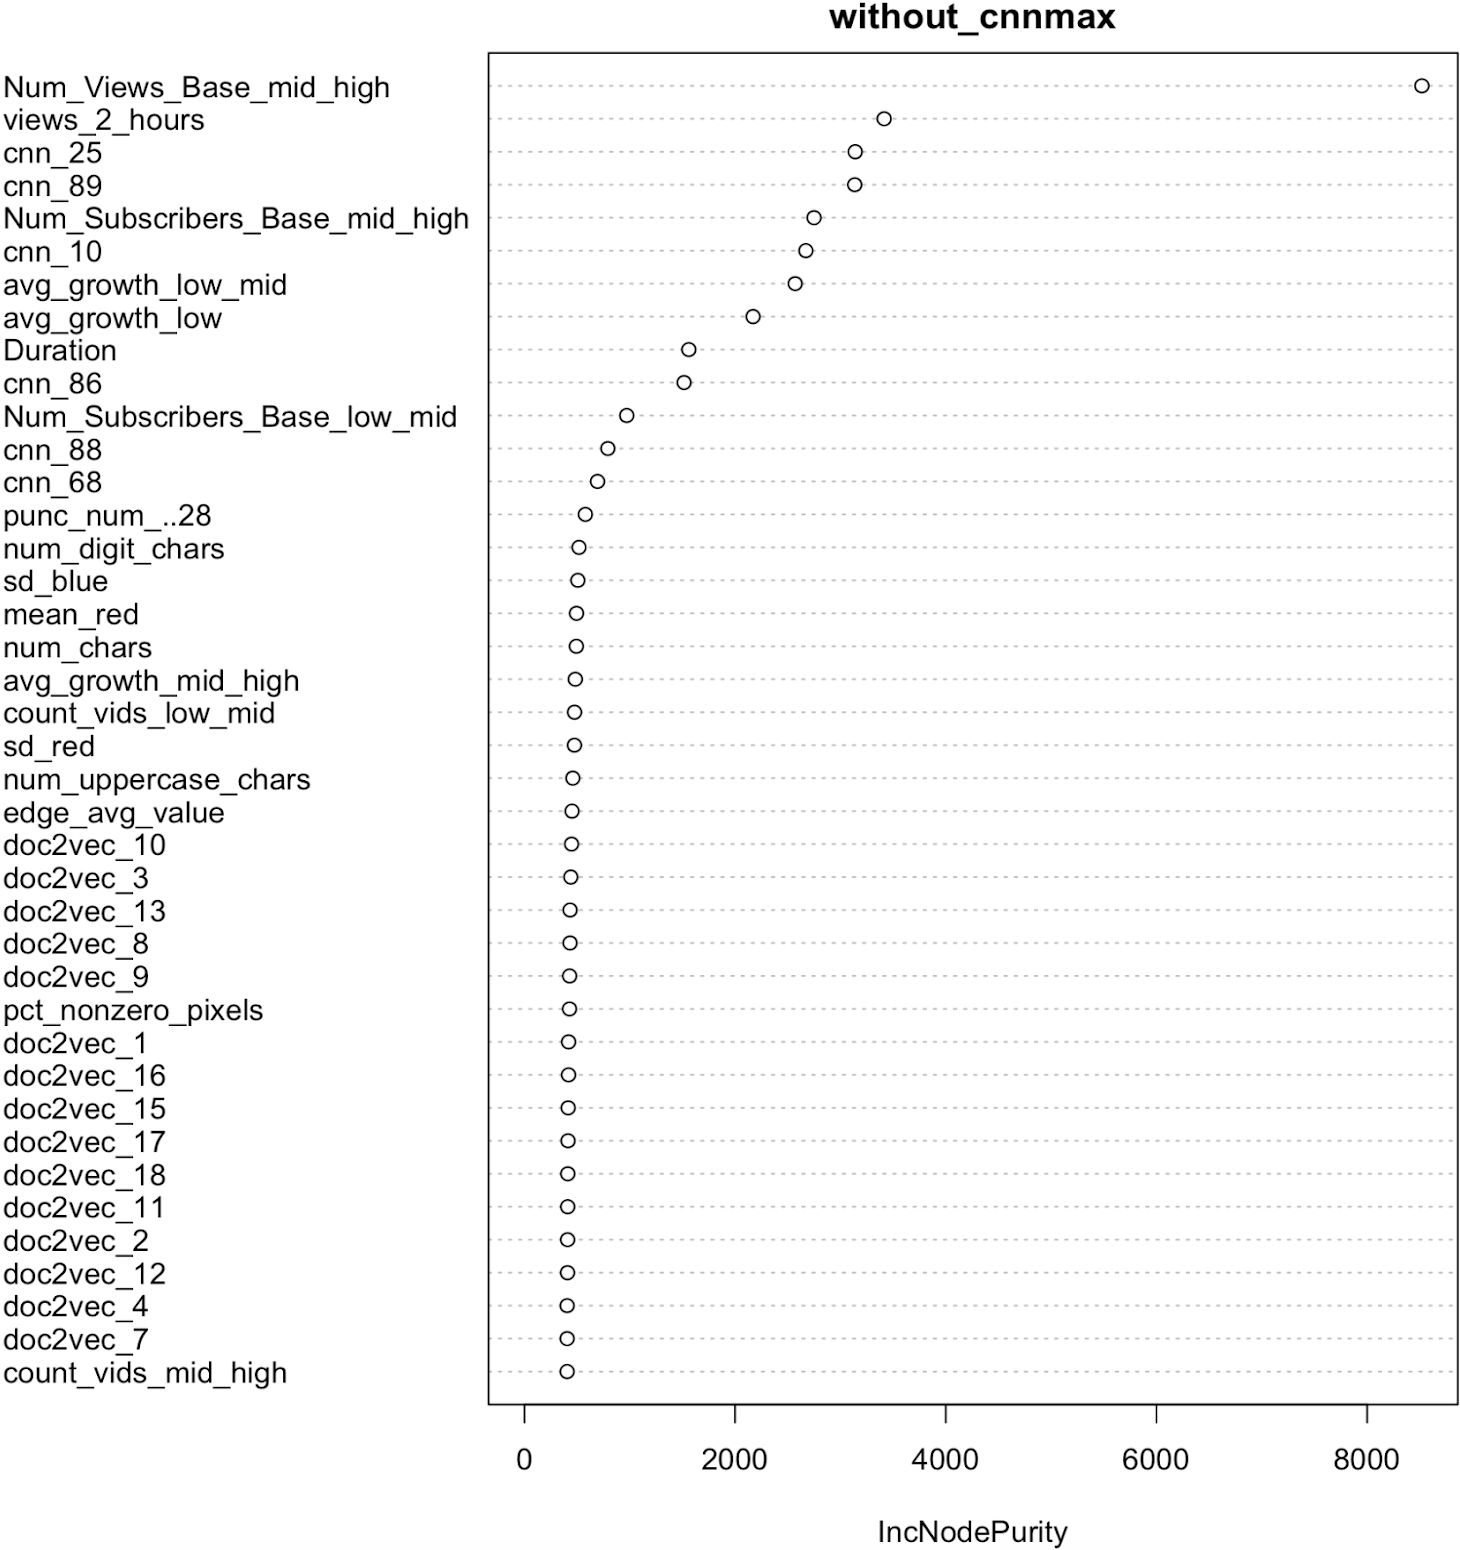
\includegraphics[width=0.75\textwidth]{varImpPlot.png}
    \caption{Variable importance plot of 40 most important variables in the final model. Variable importance measured by total decrease in node impurities from splitting on the variable, averaged over all trees.}
    \label{fig:varimp}
\end{figure}

\pagebreak

\clearpage

\subsection*{Script}

\inputminted{R}{final_final.R}

\end{document}
